\section{Implementation of Perturb and Observe algorithm}\label{MPPTImplementation}

Due to the previous mentioned advantages of the Perturb and Observe (P\&O) \todo{include in nomenclature. AT} algorithm, it was decided to implement this commonly used control algorithm for tracking the MPP. The basic operation of the P\&O algorithm consists of perturbing the operating voltage of the PV module by means of the variation of the duty cycle of the DC-DC converter. After each perturbation the power generated by the PV module is measured (observed) and stored in order to compare it with the previous value of the power. Based on the result of the comparison the MPP can be tracked by deciding if in the next perturbation the panel's voltage should be increased or decreased.

There are different techniques for implement the P\&O algorithm according to the value of the variable controlled by the MPPT and also depending if the perturb value is fixed or variable \todo{REF to "Perturb and observe MPPT technique for PV based microgrids". Stef}. The conventional P\&O algorithm uses a fixed perturb to generate a voltage or current reference signal for the outer control loop. The outer loop is usually a PI controller which controls the switching of the DC-DC converter \todo{is it really a PI?? AT}. Another way of implementing the conventional P\&O algorithm is using an adaptive perturb by setting the initial perturbation to 10\% of the open-circuit voltage ($V_{oc}$). After each iteraction its value is decreased by 50\% until it reaches 0.5\%
of $V_{oc}$. \todo{im guessing this values are made up? otherwise ref. AT} A different technique consists on using the duty cycle of the converter as the variable controlled by the MPPT block and, therefore, avoiding the PI controller. As with the conventional P\&O method this technique can also be implemented using fix or variable perturb step \todo{REF to "Perturb and observe MPPT technique for PV based microgrids". Stef}. 

The P\&O algorithm that will be implemented in this project is the \todo{a modified? AT} modified version of the conventional one and using a variable perturb step. It was decided to directly control the duty cycle to simplify the control system as it is not necessary to implement the PI controller \todo{Are we going to implement the PI controller at some point??Stef}. On the other hand, an adaptive perturb is selected instead of a fixed one because if a small perturb step is implemented the MPPT takes longer time to reach the MPP, however, using a large perturb step the tracking would be faster but the oscillations around the MPP would be higher \todo{REF to "Perturb and observe MPPT technique for PV based microgrids"Stef}. For this reason, it was decided to start with a perturbation step of 10\% of the $V_{oc}$ until the system detects the first MPP crossing \todo{check this with the final implementation in the lab?? delta D is 0.0122 for 0.45V increment/decrement. Stef}. At this point the perturbation step is iteractively reduced to half of its previous value in order to reach accurately the MPP with lower oscillations \todo{Write about the final implementation of the step(minimum value so we don't get 0). Stef}. Figure \ref{BD_POalgorithm} shows the implementation of the system in \textit{PLECS} including the MPPT controller unit which operates at a frequency of 100 Hz. 

\begin{figure}[H]
	\begin{center}
		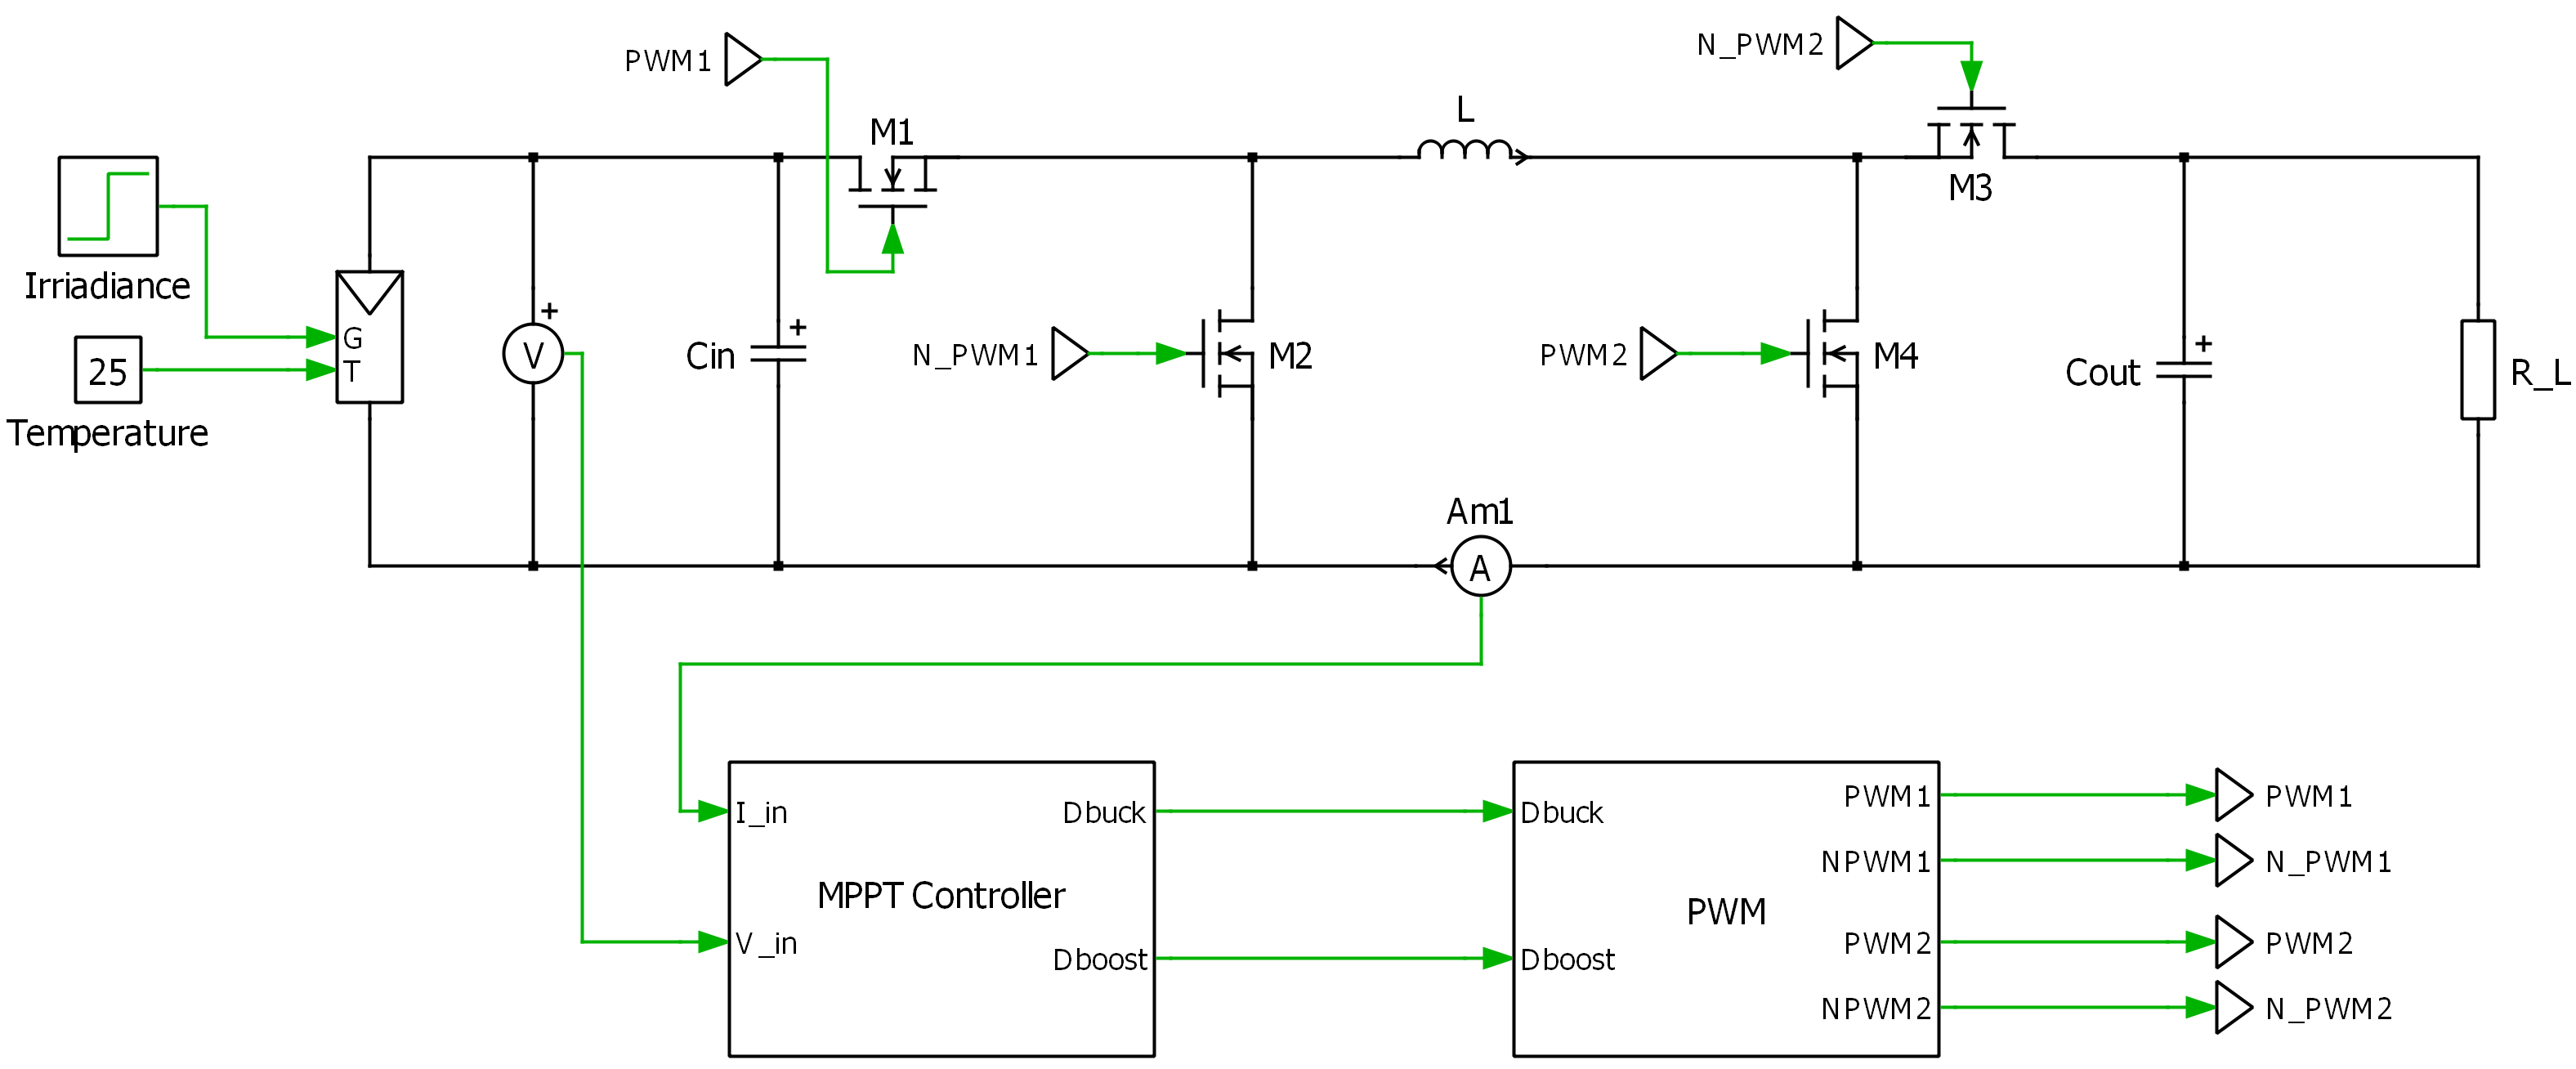
\includegraphics[width=\textwidth]{../Pictures/BD_implementation_POalgorithm}
		\caption{Block diagram of the system including the MPPT.}\todo{change this figure! Stef}
		\label{BD_POalgorithm}
	\end{center}	
\end{figure}

From the previous figure it is observed that the output of the MPPT is a duty cycle which is send to another block called "Mode decision" \todo{i don't think this variable should be called duty cycle. AT}. This block is used to decide if the DC-DC converter operates in buck or in boost mode. The transfer function of the converter when it is operating in buck and in boost mode is shown in equations \ref{tfbuck} and \ref{tfboost}, respectively. Plotting this transfer functions in figure \ref{fig:tfmodes} and mapping them as shown in figure \ref{fig:modedecisionmapping} it is possible to obtain the corresponding duty cycle for the buck or the boost mode. If the duty cycle from the MPPT \todo{Not duty cycle!! Call it different: control variable,valg... Stef, +1 AT} is lower than 0.5 (D<0.5) means that the output voltage is lower than the input voltage and thus the converter will work as a buck converter with duty cycle $D_{buck}=2\cdot D$. On the other hand, if $D \geq 0.5$ means that the output voltage is higher or equal than the input voltage and, therefore, the converter will operate in boost mode with duty cycle $D_{boost}=2\cdot D - 1$.\todo{Even though it was a big issue of the design of the program i don't think it is important to specify how the decision is taken. Maybe better to say "With the variables blabla and blabla the decision is taken wether to work on buck or boost mode" or something like that, otherwise it is not going to be understood. AT} These duty cycles are used to generate the corresponding PWM signals according to the converter's mode of operation at each time. 

\vspace{1cm}
\begin{minipage}{0.3\linewidth}
	\begin{equation}
	\frac{V_o}{V_i} = D
	\end{equation}
	\label{tfbuck}
\end{minipage}%
\begin{minipage}{0.5\linewidth}
	\begin{equation}
	\frac{V_o}{V_i}= \frac{1}{1-D}
	\end{equation}
	\label{tfboost}
\end{minipage}

\begin{figure}[H]
	\begin{minipage}[b]{0.9\linewidth}
		\centering
		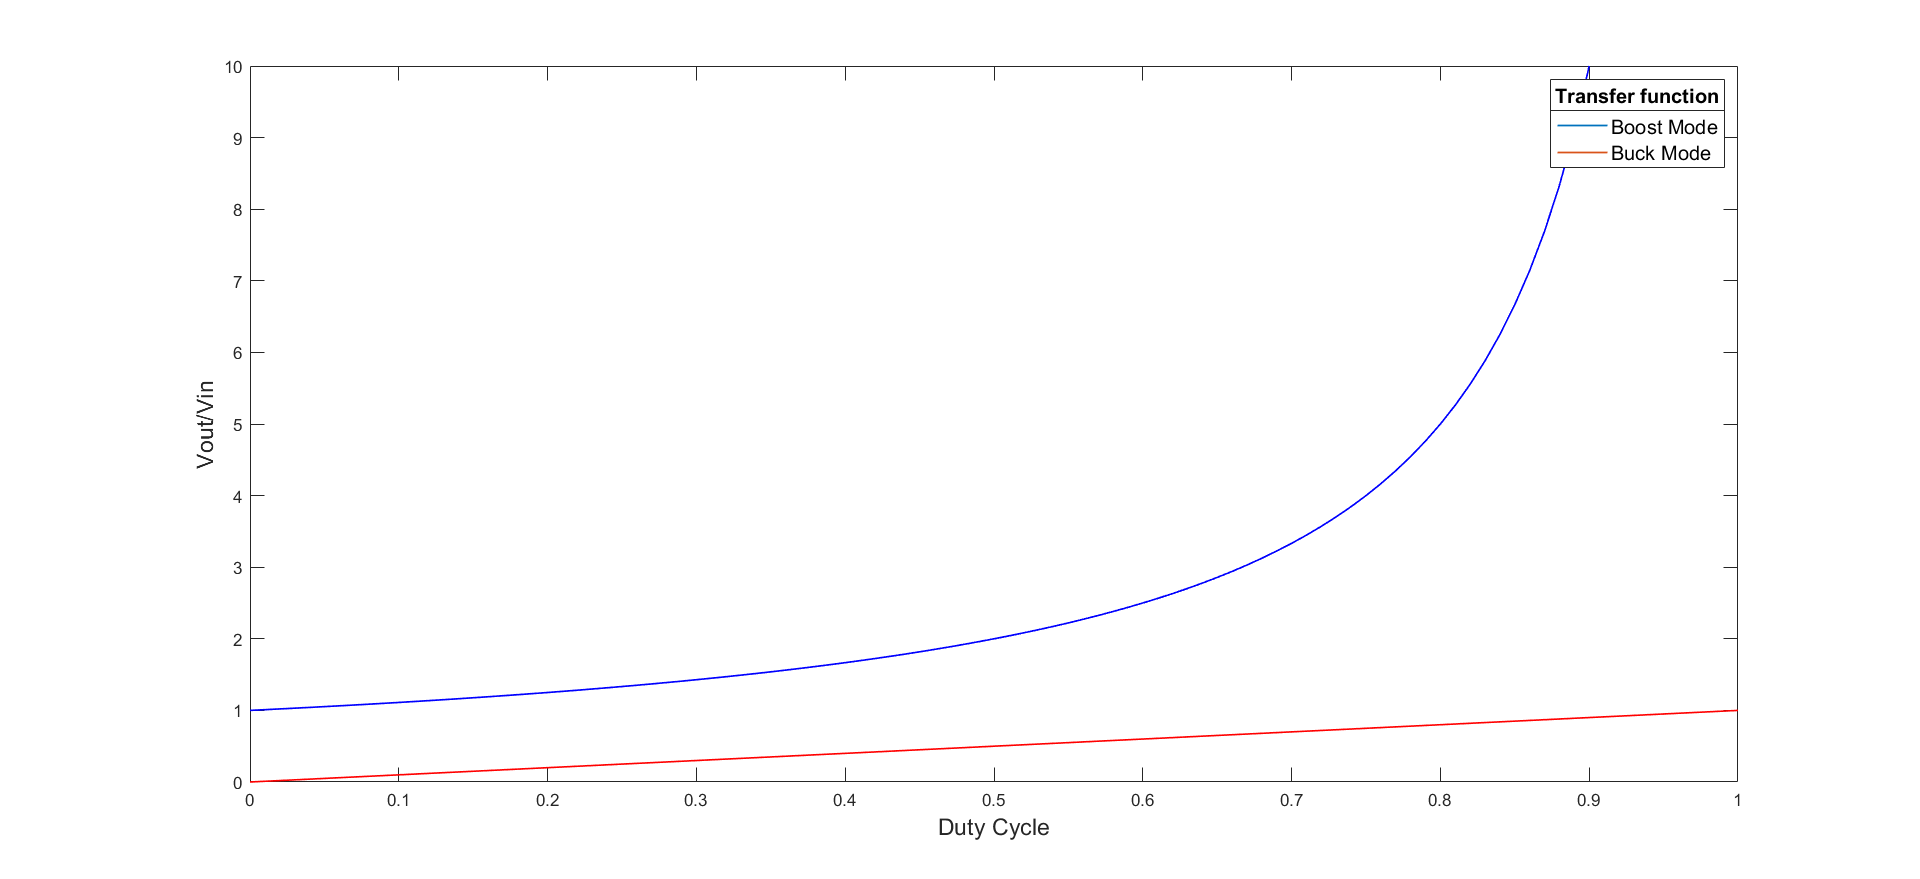
\includegraphics[width=\textwidth]{../Pictures/transfer_function_buck_boost_mode}
		\caption{Transfer function of buck mode and boost mode.}
		\label{fig:tfmodes}
	\end{minipage}
	\hspace{0.5cm}
	\begin{minipage}[b]{0.9\linewidth}
		\centering
		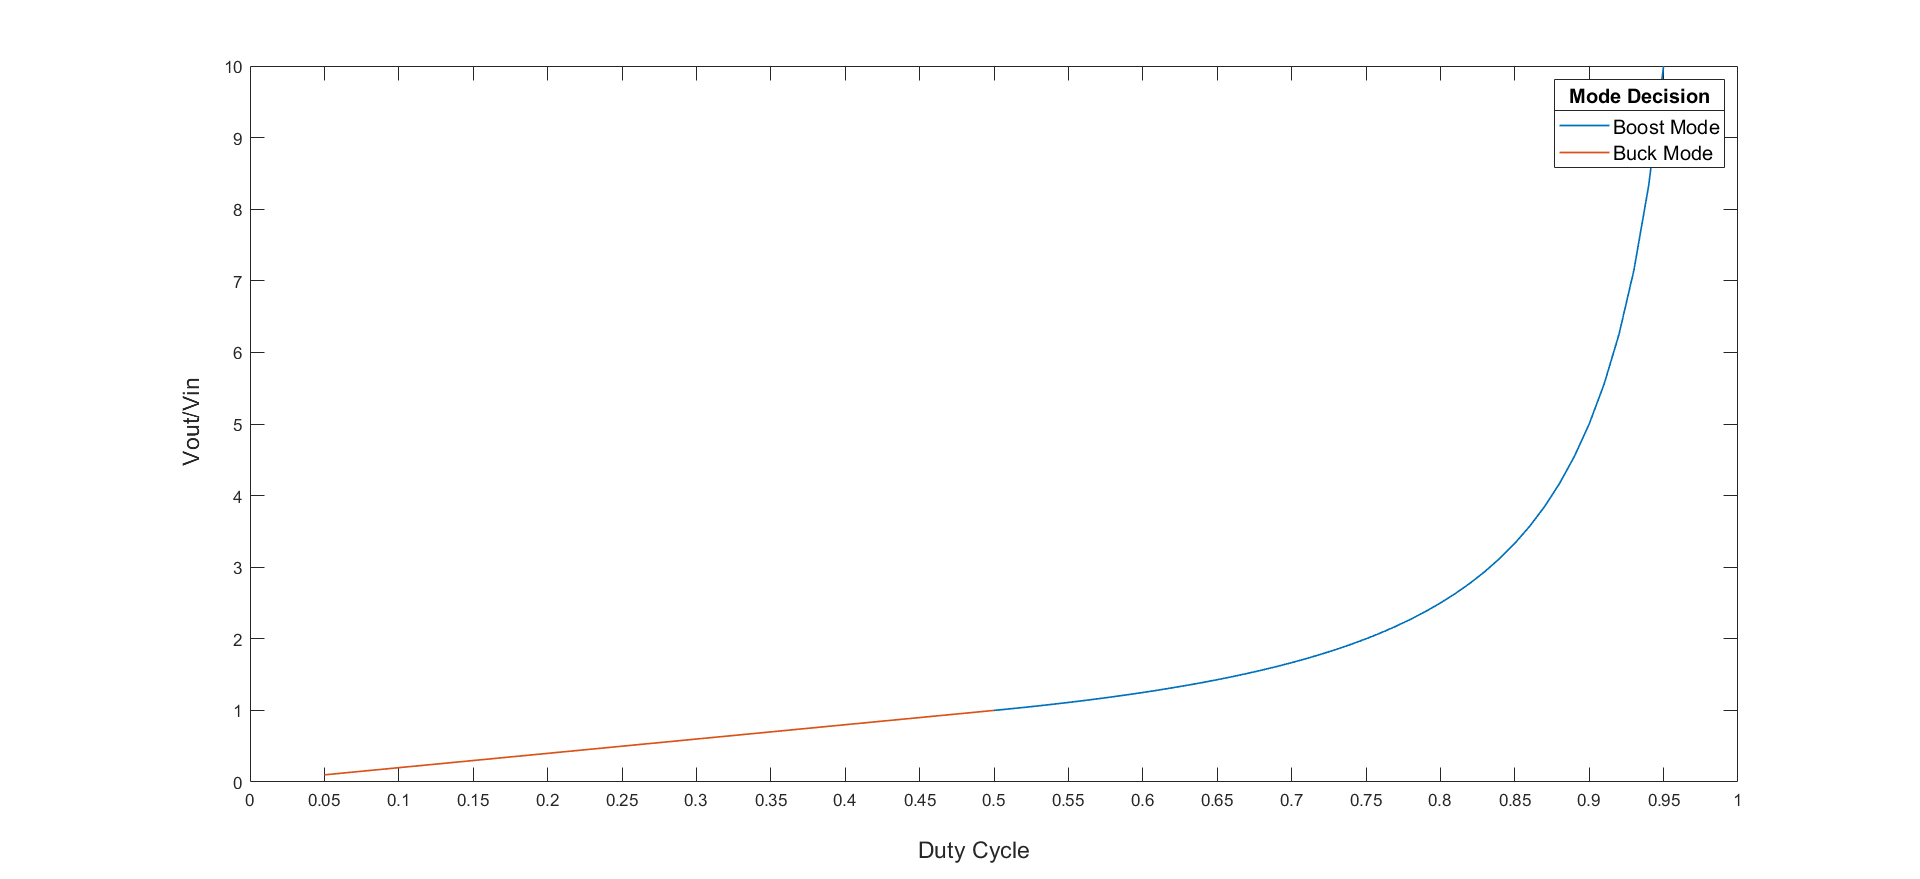
\includegraphics[width=\textwidth]{../Pictures/Mode_decision_duty_vs_gain}
		\caption{Mapping to decide the mode of operation.}\todo{change the x axis name. Stef}
		\label{fig:modedecisionmapping}
	\end{minipage}
\end{figure}


The corresponding flow chart used for the implementation of the Perturb \& Observe algorithm is shown in figure \ref{fcfinal}.


\begin{figure}[H]
	\begin{center}
		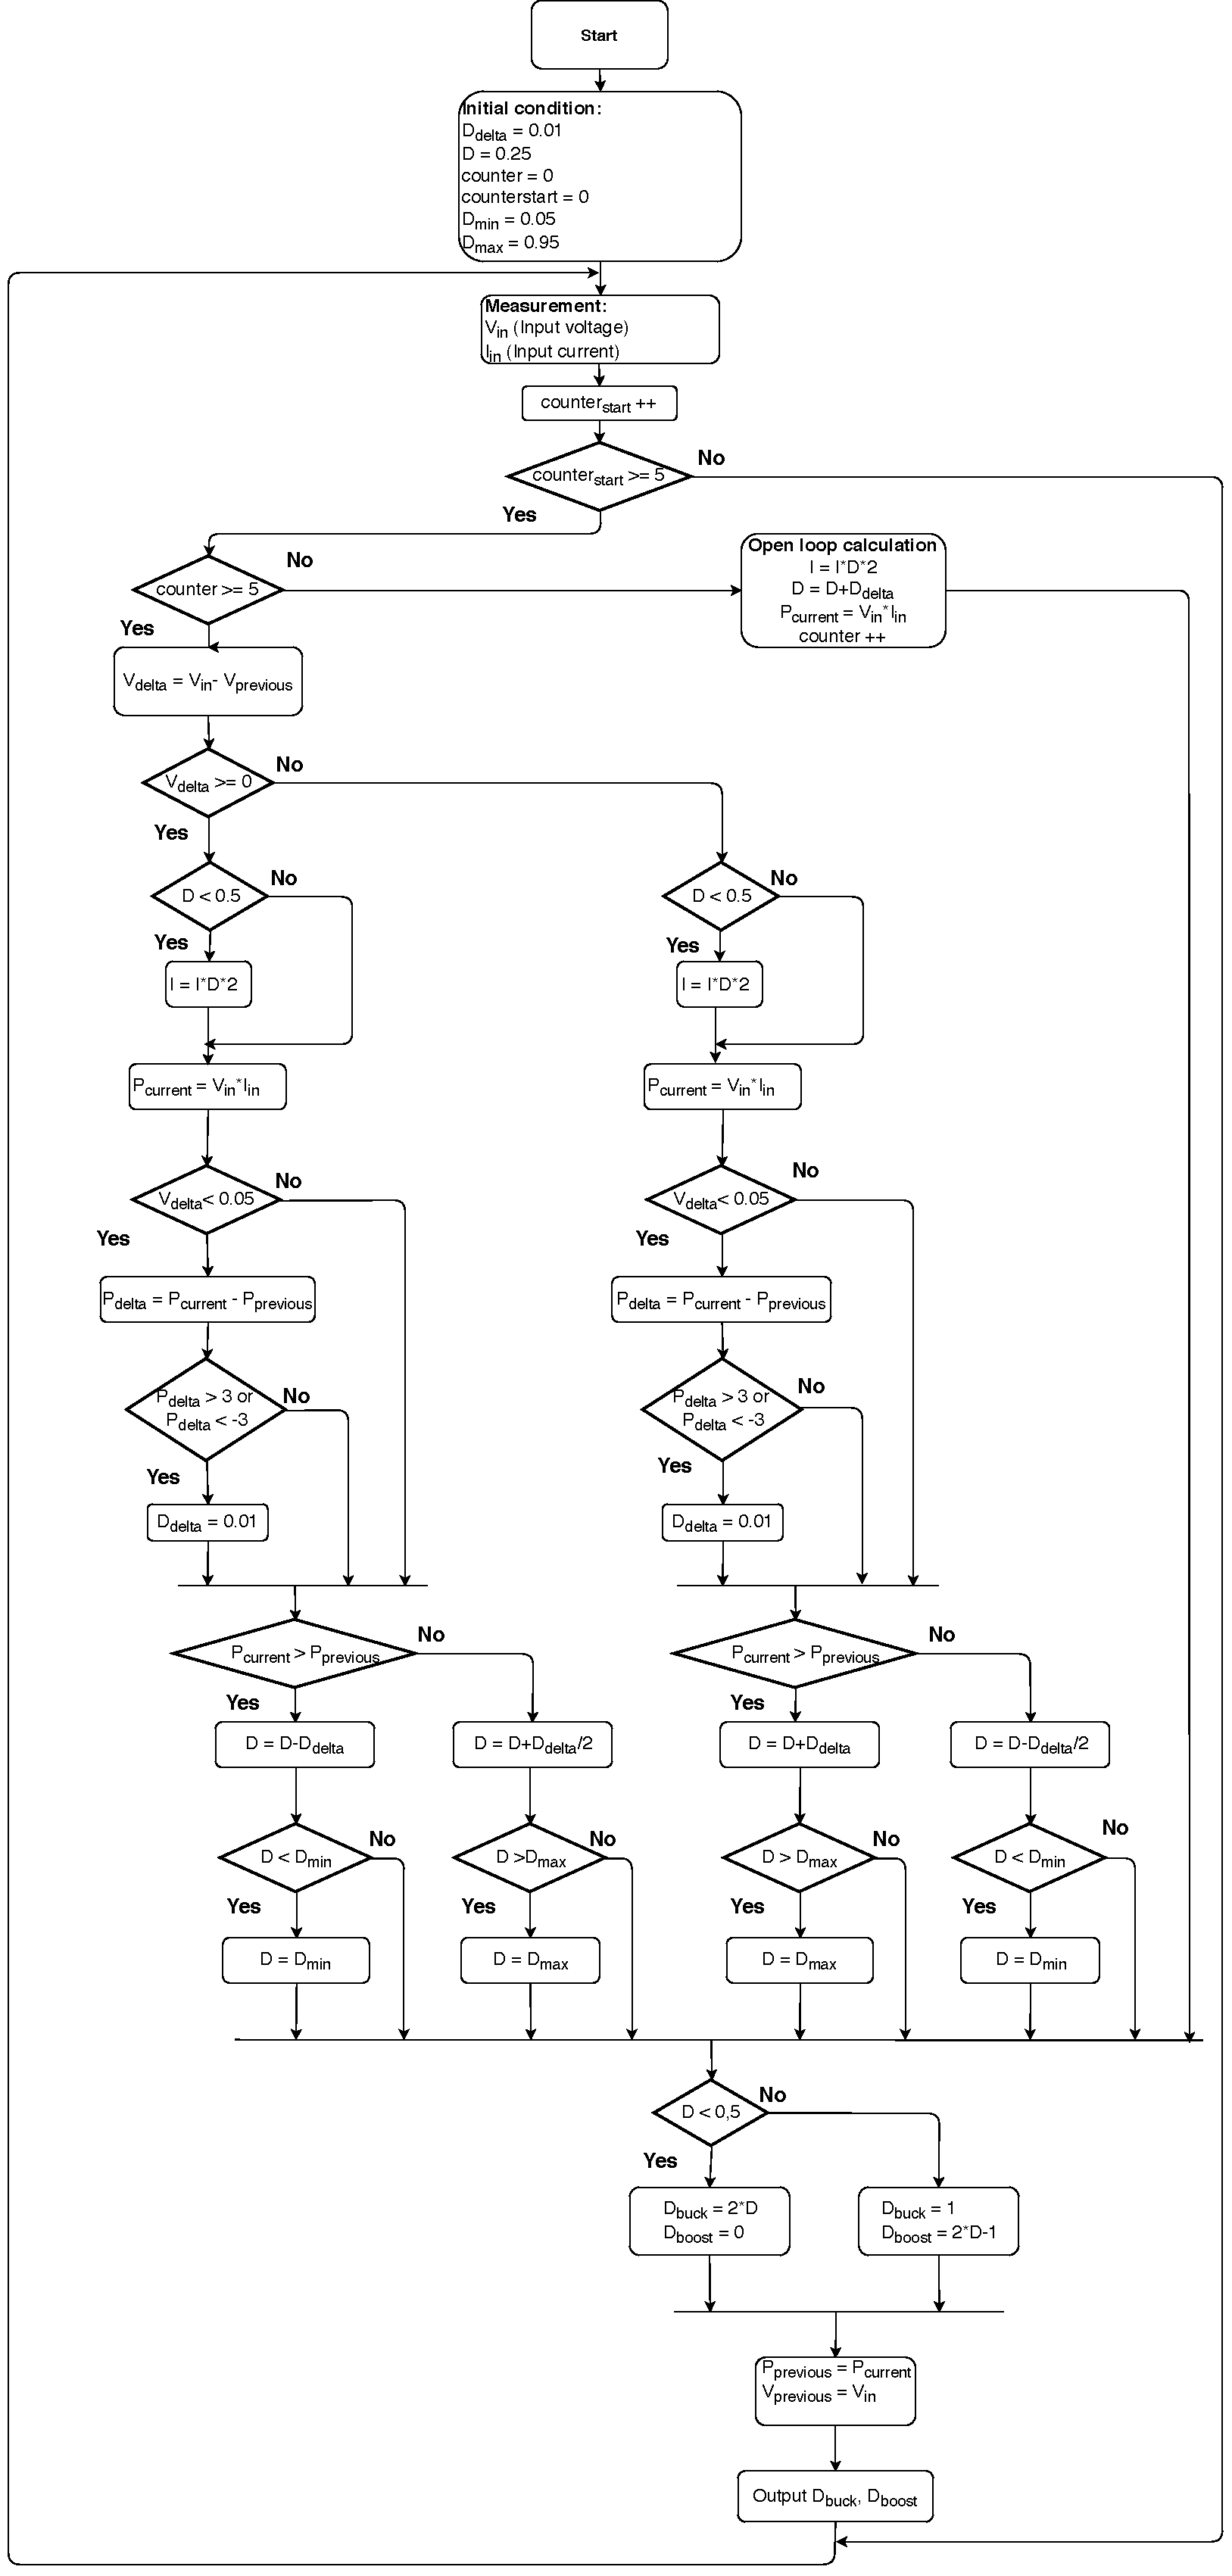
\includegraphics[width=0.8\textwidth]{../Pictures/P1/Flow_chart/2018_11_15_Flow_chart_MPPT_Buck-Boost_converter}
		\caption{Flow chart for the Perturb \& Observe algorithm.}
		\label{fcfinal} \todo{modify the flow chart once we have the final! Stef}
	\end{center}	
\end{figure}

From the flow chart it can be observed that the MPPT is enabled after five sample times to ensure that the panel's voltage has reached the value of the open-circuit voltage $V_{oc}=45 V$ before starting the comparison of the voltage measurements.
It is important to notice from figure \ref{BD_POalgorithm} that the current measurement is carried out in the inductor instead of in the PV panel. This is done for possible future implementation of an outer PI control loop. For this reason, it is necessary to transform the measured current in order to get the corresponding measurement for the PV module's current. This current transformation is just necessary in the case of buck mode as explained in section \ref{current_sensor}. The MPPT evaluates if the converter is working in buck mode and if it is, it multiplies the measured current by the corresponding duty cycle $D_{buck}=2\cdot D$\todo{change D for control variable (check everywhere)}. In boost mode the average current through the inductor corresponds to the PV module's current. 


The operation of the algorithm, shown in figure \ref{fcfinal}, is an iterative process in which the values of the PV panel's voltage and power, before and after applying a voltage perturbation, are compared  in order to locate the point of operation. This way it is possible to decide if the panel's voltage has to be increased or decreased in order to achieve the MPP. Based on the PV characteristic curve shown in figure \ref{fig:mpp}, the following situations can occur:

\begin{enumerate}
\item Increment of voltage and increment of power means that the point of operation is located to the left of the MPP. Therefore, the perturbance continues in the same direction (voltage is increased) with a fixed perturb step. 
\item Increment of voltage and decrement of power means that the point of operation of the panel has gone from being located to the left of the MPP to the right of it. Therefore, the next perturbance is in the opposite direction (voltage is decreased) with a perturb step half of the previous step value.
\item Decrement of voltage and increment of power means that the operation point is located to the right of the MPP. Therefore, the perturbance continues in the same direction (voltage is decreased) with a fixed perturb step. 
\item Decrement of voltage and decrement of power means that the point of operation of the panel has changed from being located to the right of the MPP to the left of it. Therefore, the next perturbance is in the opposite direction (voltage is increased) with a perturb step half of the previous step value.
\end{enumerate}
\todo{I really like this way of explaining the algorithm. AT}

After the process, once the MPP has been reached, the algorithm oscillates around this optimal point of operation. However in this case, as a variable perturb step is applied, the oscillations around the MPP will be much lower than using fixed perturb step.  


\iffalse
THINGS TO CHANGE IN THE ALGORITHM (code and flow chart):
\begin{itemize}
	\item Dmin=0.05 and Dmax=0.95 not necessary as D is not duty cycle! Check everywhere to change D for control variable. 
	\item Logic for the reset of deltaD when the system detects a change in irradiance. I think we shouldn't include this condition in the flow chart we can just show the results in graphs (in the next section) and we make the flow chart easier to read and just showing the main code. 
	\item Not necessary the start counter because with the counter for the open loop calculation the MPPT is enabled after the Voc has been reached. 
\end{itemize}
\fi


